%%%%%%%%%%%%%%%%%%%%%%%%%%%%%%%%%%%%%%%%%%%%%%%%%%%%%%%%%%%
% Slides for Protein-Protein Interaction Network Analysis
% Social Network Analysis, MIMUW 2026
% Agata Kopec, 469385
%%%%%%%%%%%%%%%%%%%%%%%%%%%%%%%%%%%%%%%%%%%%%%%%%%%%%%%%%%%

\documentclass[aspectratio=169]{beamer}
\usetheme{metropolis}

\usepackage{graphicx}
\usepackage{booktabs}
\graphicspath{{../results/figures/}}

% Accent color overrides for the metropolis theme.
\definecolor{myaccent}{HTML}{C0306E}
\setbeamercolor{frametitle}{bg=myaccent, fg=white}
\setbeamercolor{progress bar}{fg=myaccent}
\setbeamercolor{title separator}{fg=myaccent}
\setbeamercolor{progress bar in head/foot}{fg=myaccent}
\setbeamercolor{progress bar in section page}{fg=myaccent}
\setbeamercolor{alerted text}{fg=myaccent}

\title{Protein-Protein Interaction Network Analysis for Endometriosis}
\subtitle{Social Network Analysis course final project}
\author{Agata Kope\'c, 469385}
\institute{Faculty of Mathematics, Informatics and Mechanics\\University of Warsaw}
\date{May 2026}

\begin{document}

\maketitle



\begin{frame}{Research questions}
  \begin{itemize}
    \item Which set of $k$ proteins, blocked together, best limits the spread of the disease signal?
    \item Does the optimal set depend on the chosen algorithm?
  \end{itemize}
\end{frame}




\begin{frame}{Methodology}
Diffusion models:
  \begin{itemize}
    \item Susceptible-Infected-Recovered (SIR),
    \item Independent Cascade (IC).
  \end{itemize}

  \vspace{0.5em}

Blocking algorithms:
  \begin{itemize}
    \item group centrality: greedy group degree, greedy iterative betweenness,
    \item influence maximization: greedy, run under SIR and IC
  \end{itemize}
\end{frame}




\begin{frame}{Data Sources and Network Construction}
  Endometriosis Genes from DisGeNET: https://disgenet.com
  \begin{itemize}
    \item Filters: UMLS C0014175, confidence score $\ge 0.25$, 166 genes total
  \end{itemize}
  Protein graph from STRING database: https://string-db.org
  \begin{itemize}
    \item Filters: confidence score $\ge 0.4$, first-shell expansion, dropped weights
  \end{itemize}
\end{frame}



\begin{frame}{Network Results}
  \begin{itemize}
    \item unweighted,
    \item undirected,
    \item connected,
    \item 454 nodes,
    \item 21,095 edges,
    \item average degree $\approx$ 93,
    \item density $\approx$ 0.205
  \end{itemize}
\end{frame}





\begin{frame}{Null models}
  Random networks as a control group, all share $V = 454$.

  \vspace{0.5em}

  \begin{itemize}
    \item Erd\H{o}s-R\'enyi
    \item Barab\'asi-Albert
    \item Configuration model
  \end{itemize}
\end{frame}



\begin{frame}{Network statistics}
  \centering
  \begin{tabular}{lrrrr}
    \toprule
     & $|E|$ & Density & Clustering & $\bar{\ell}$ \\
    \midrule
    PPI & 21{,}095 & 0.205 & 0.637 & 1.94 \\
    ER  & 21{,}253 & 0.207 & 0.206 & 1.79 \\
    BA  & 21{,}253 & 0.207 & 0.298 & 1.79 \\
    CM  & 21{,}095 & 0.205 & 0.512 & 1.84 \\
    \bottomrule
  \end{tabular}

  \vspace{1em}

  PPI clustering stands out
\end{frame}



\begin{frame}{Degree distribution}
  \centering
  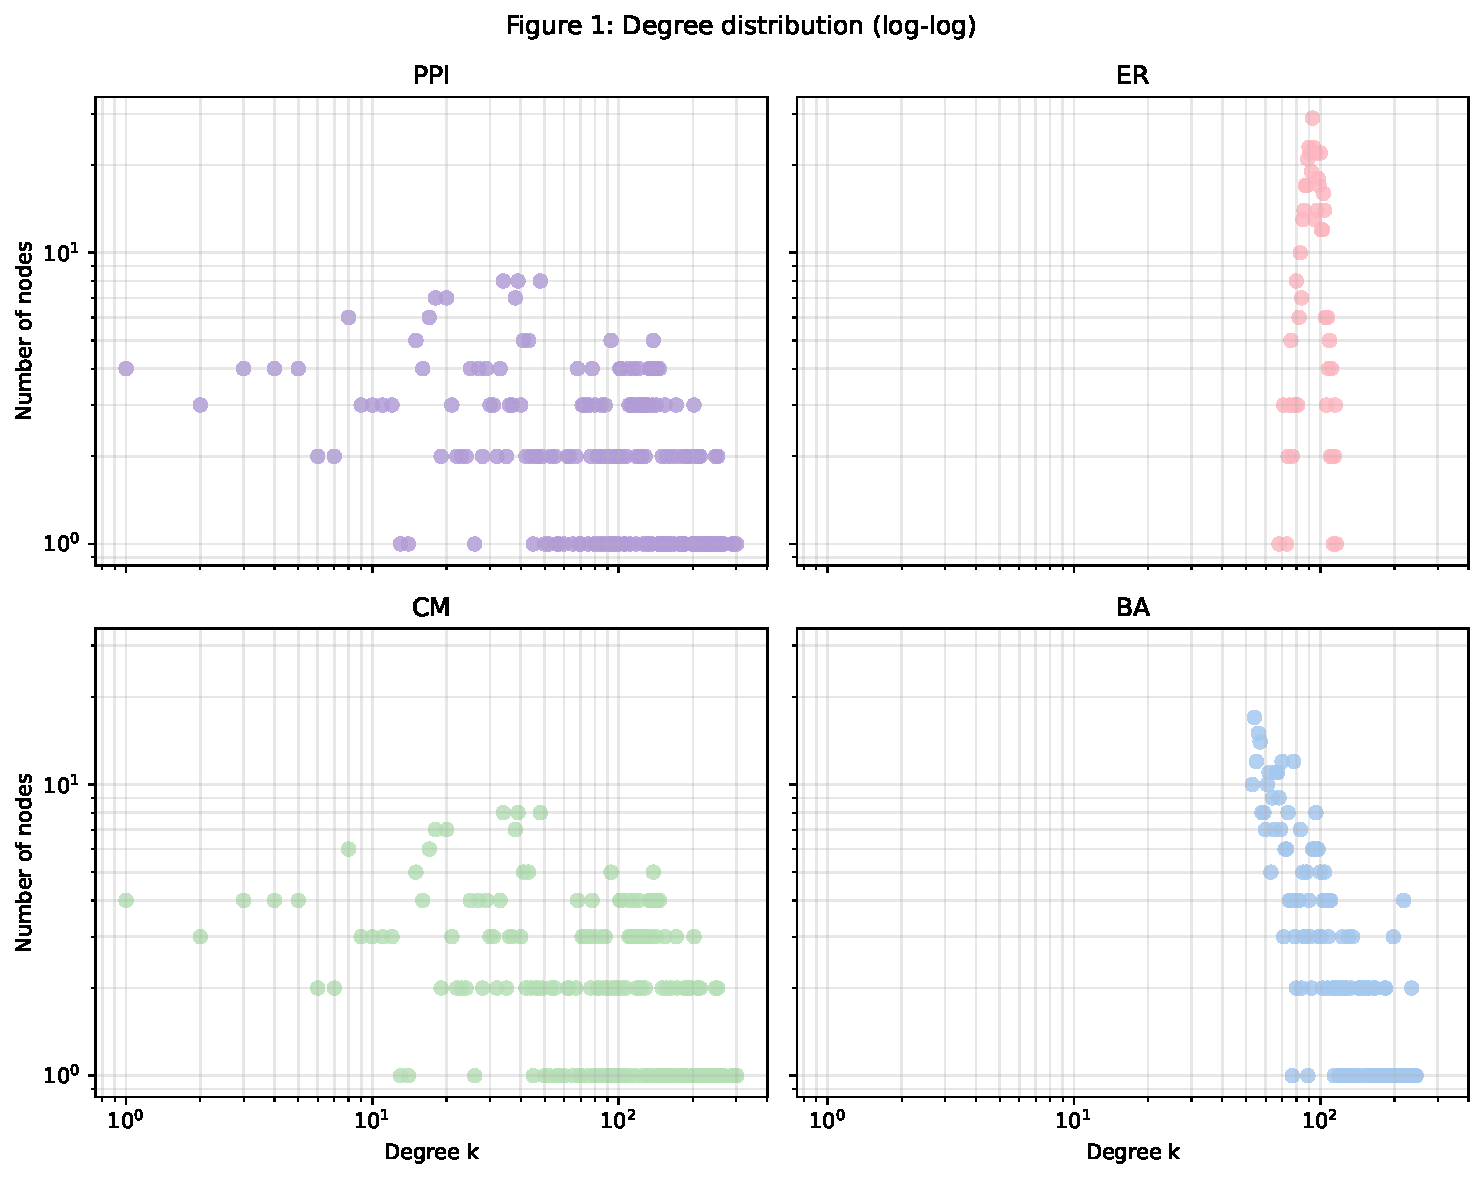
\includegraphics[height=0.75\textheight,keepaspectratio]{fig1_degree_distribution.pdf}

  \vspace{0.3em}

  PPI and CM heavy-tailed; ER narrow Poisson; BA power-law;
\end{frame}



\begin{frame}{Diffusion models}
  Simulate the disease signal spreading and score blocking strategies by how much they reduce propagation.

  \vspace{0.5em}

  Spread reduction $= 1 - \dfrac{\text{spread for the blocked network}}{\text{spread for the unblocked network}}$

  \vspace{0.5em}

  \begin{itemize}
    \item SIR, Susceptible-Infected-Recovered: infection rate $\beta$, recovery rate $\gamma$.
    \item IC, Independent Cascade: activation probability $p$.
  \end{itemize}
\end{frame}



\begin{frame}{Diffusion models' calibration}
  Calibrate $\beta$, $\gamma$, $p$ so that unblocked propagation reaches around 70\% of the network.

  \vspace{0.5em}

  \centering
  \begin{tabular}{lrr}
    \toprule
    Parameters & Mean spread & \% of network \\
    \midrule
    SIR $\beta=0.005, \gamma=0.20$ & 318.7 & 70 \\
    SIR $\beta=0.010, \gamma=0.20$ & 382.3 & 84 \\
    SIR $\beta=0.020, \gamma=0.20$ & 418.6 & 92 \\
    SIR $\beta=0.050, \gamma=0.20$ & 439.5 & 97 \\
    IC $p=0.005$  &  59.9 & 13 \\
    IC $p=0.010$  & 170.5 & 38 \\
    IC $p=0.020$  & 294.7 & 65 \\
    IC $p=0.050$  & 386.0 & 85 \\
    \bottomrule
  \end{tabular}

  \vspace{0.5em}

  Chosen: $\beta = 0.005$, $\gamma = 0.20$, $p = 0.02$.
\end{frame}



\begin{frame}{Blocking algorithms}
  Three algorithms choose the proteins to block: two group-centrality and one influence-maximization.

  \vspace{0.5em}

  \begin{itemize}
    \item \texttt{gdeg}, greedy group degree: removing hubs,
    \item \texttt{gbtw}, greedy iterative betweenness: removing bridges,
    \item \texttt{gim}, greedy influence maximization: reducing spread
  \end{itemize}

  \vspace{0.5em}

  \texttt{gim} runs twice, once under SIR and once under IC.
\end{frame}



\begin{frame}{Top 10 picks per chain}
  \centering
  \begin{tabular}{rllll}
    \toprule
     & \texttt{gdeg} & \texttt{gbtw} & \texttt{gim\_sir} & \texttt{gim\_ic} \\
    \midrule
    1  & IL6     & ALB   & FGF4     & CD40    \\
    2  & ESR1    & ESR1  & KDR      & LAG3    \\
    3  & AKR1C3  & EGFR  & UGT1A7   & CX3CL1  \\
    4  & NCOA1   & IL6   & VTN      & HDAC2   \\
    5  & EGFR    & GAPDH & IL17A    & MED4    \\
    6  & INS     & TNF   & NTRK3    & UGT2B11 \\
    7  & ITGB3   & IL1B  & PDGFRB   & MED14   \\
    8  & APOE    & INS   & SERPINF1 & CCL13   \\
    9  & CTNNB1  & AKT1  & EREG     & PTPRC   \\
    10 & CYP3A4  & ACTB  & TIMP1    & COPS2   \\
    \bottomrule
  \end{tabular}

  \vspace{0.4em}

  {\footnotesize ESR1: estrogen receptor; FGF4, KDR: angiogenesis; CD40: immune.}
\end{frame}



\begin{frame}{Spread reduction across strategies}
  \centering
  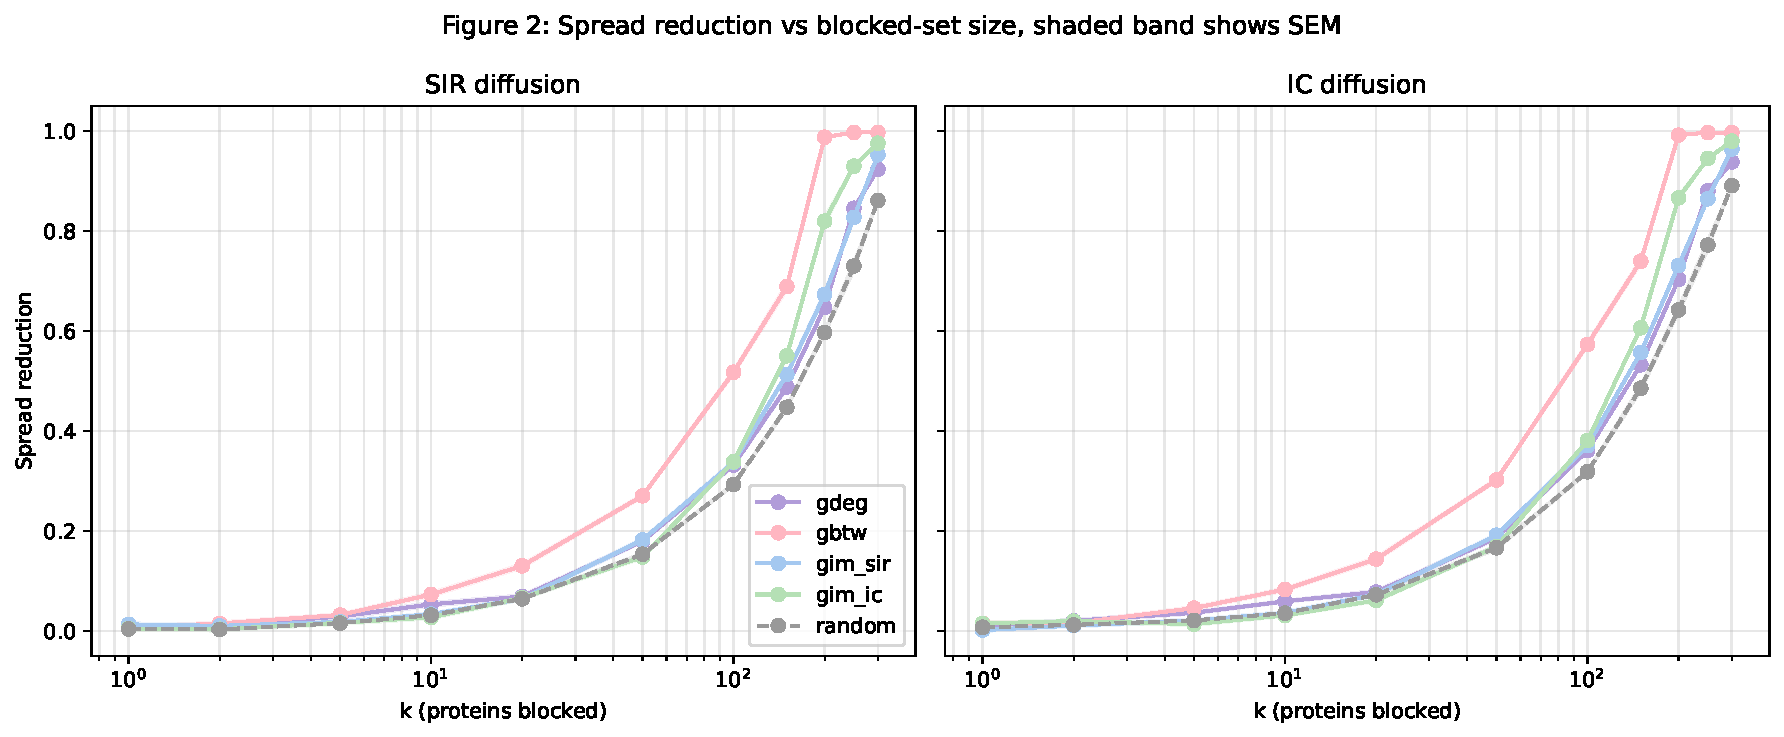
\includegraphics[height=0.75\textheight,keepaspectratio]{fig2_spread_reduction.pdf}

  \vspace{0.3em}

  \texttt{gbtw} dominates; saturates at $k \approx 200$ with 99\% reduction.
\end{frame}



\begin{frame}{PPI vs null networks}
  \centering
  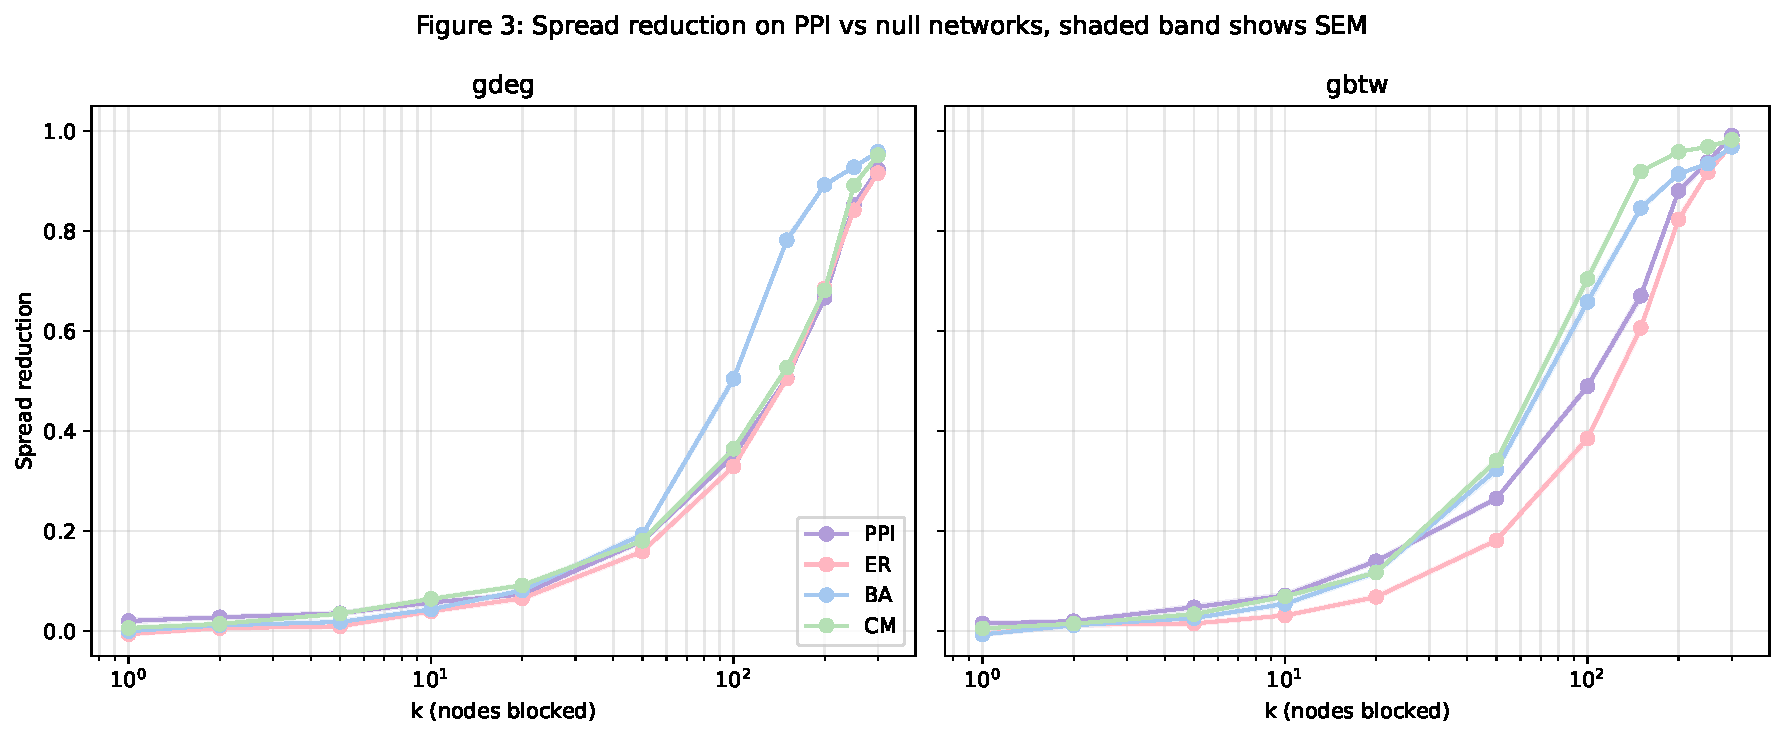
\includegraphics[height=0.75\textheight,keepaspectratio]{fig3_ppi_vs_nulls.pdf}
\end{frame}



\begin{frame}{Top-20 composition}
  \centering
  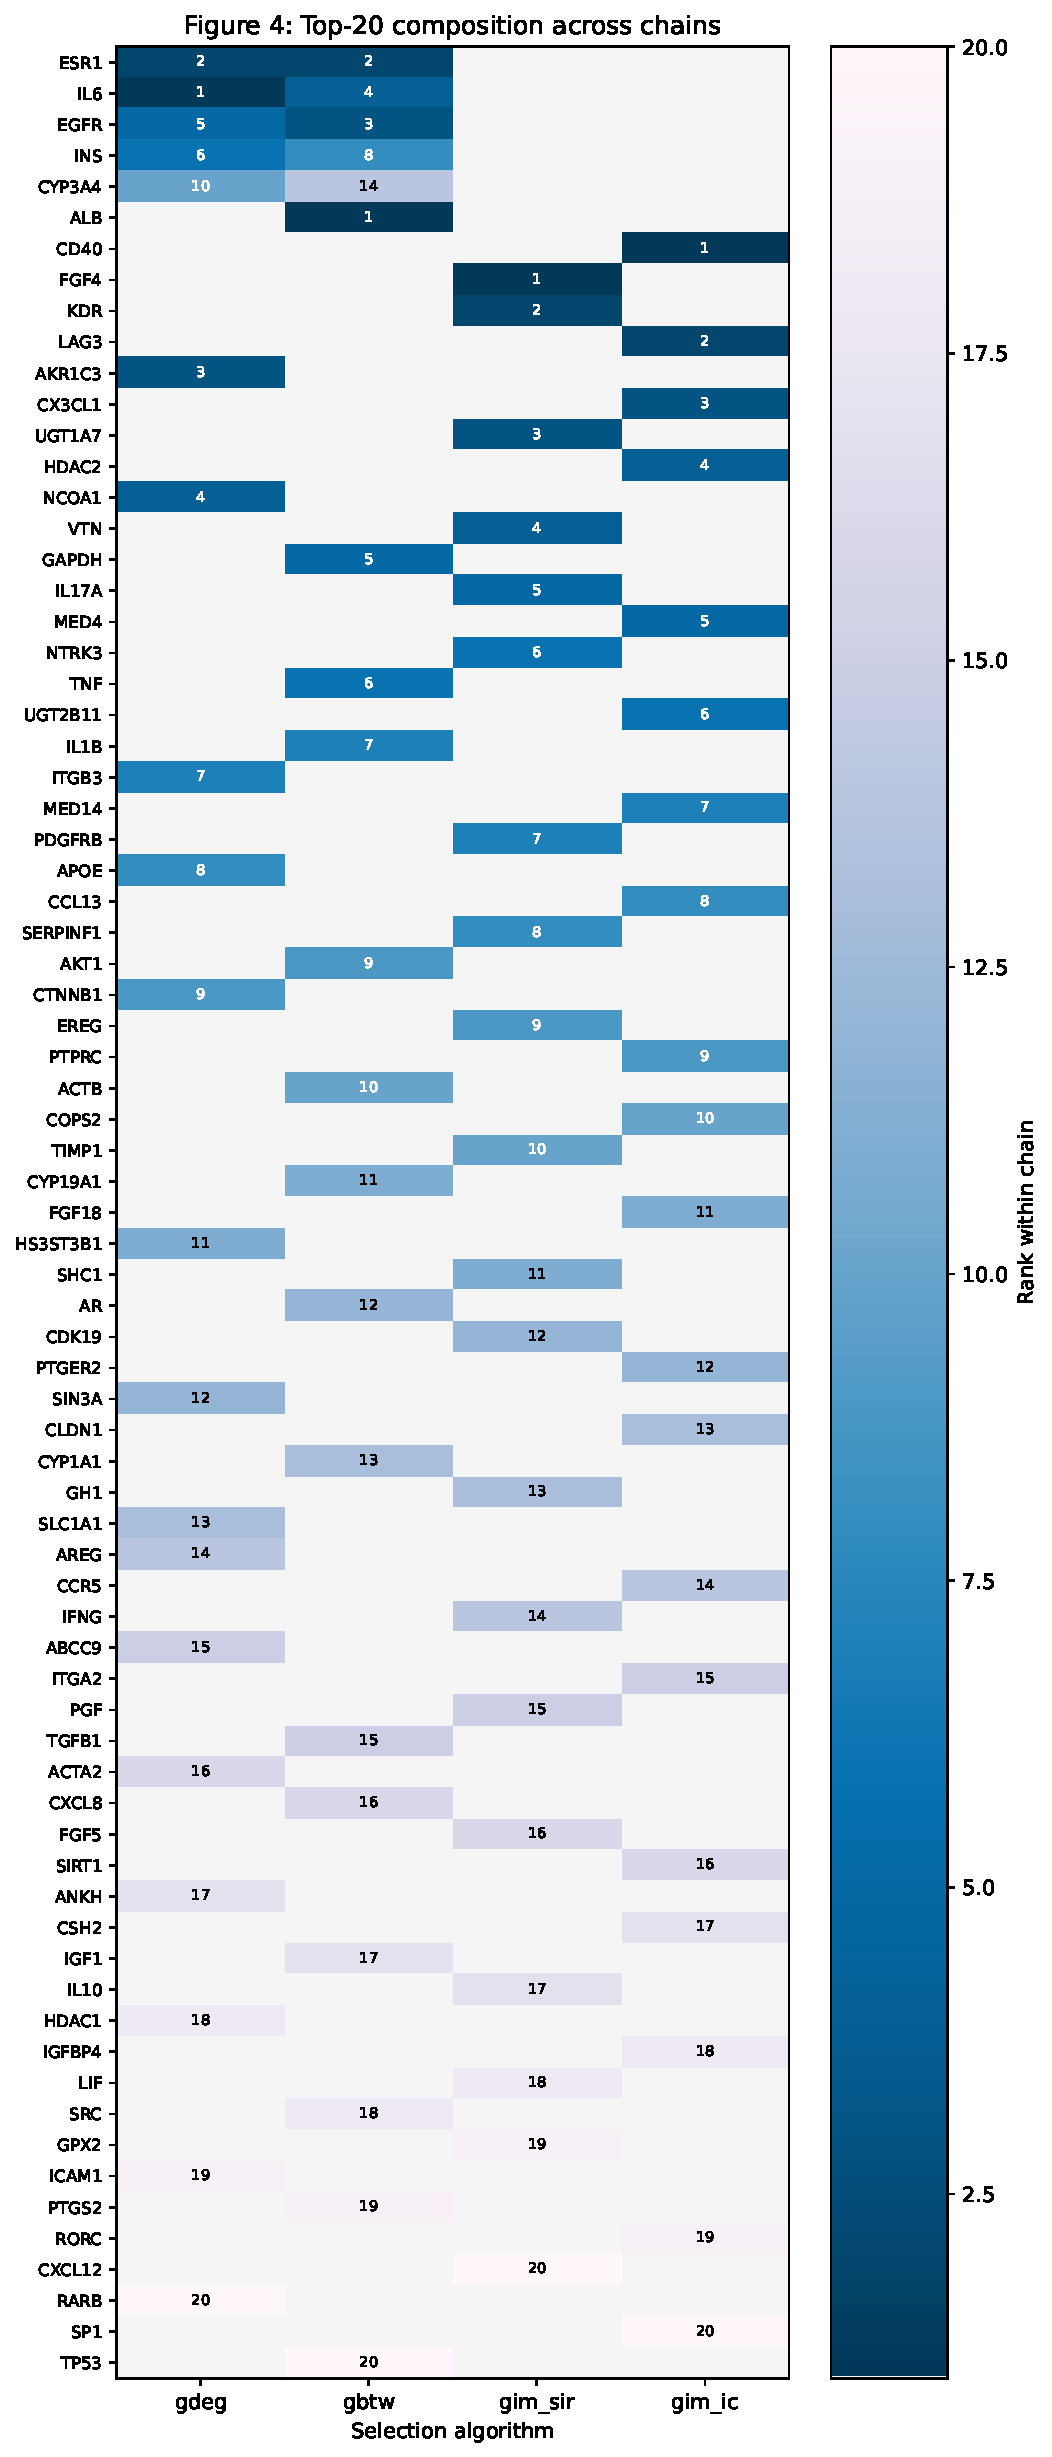
\includegraphics[height=0.75\textheight,keepaspectratio]{fig4_topk_composition.pdf}

  \vspace{0.3em}

  75 distinct proteins; only 5 shared by 2+ chains; 93\% algorithm-specific.
\end{frame}



\begin{frame}{Conclusion}
  The answer to the research question:

  \begin{itemize}
    \item Best $k$-set: prefix of the \texttt{gbtw} chain, saturates near $k = 200$
    \item Strongly algorithm-dependent: 93\% of top-20 picks are algorithm-specific
  \end{itemize}

  \vspace{0.5em}

  At a realistic small $k$, partial blocking reduction is not significant at all.
\end{frame}

\end{document}
